\documentclass{standalone}
\usepackage{tikz}
\usetikzlibrary{patterns, positioning}


\begin{document}
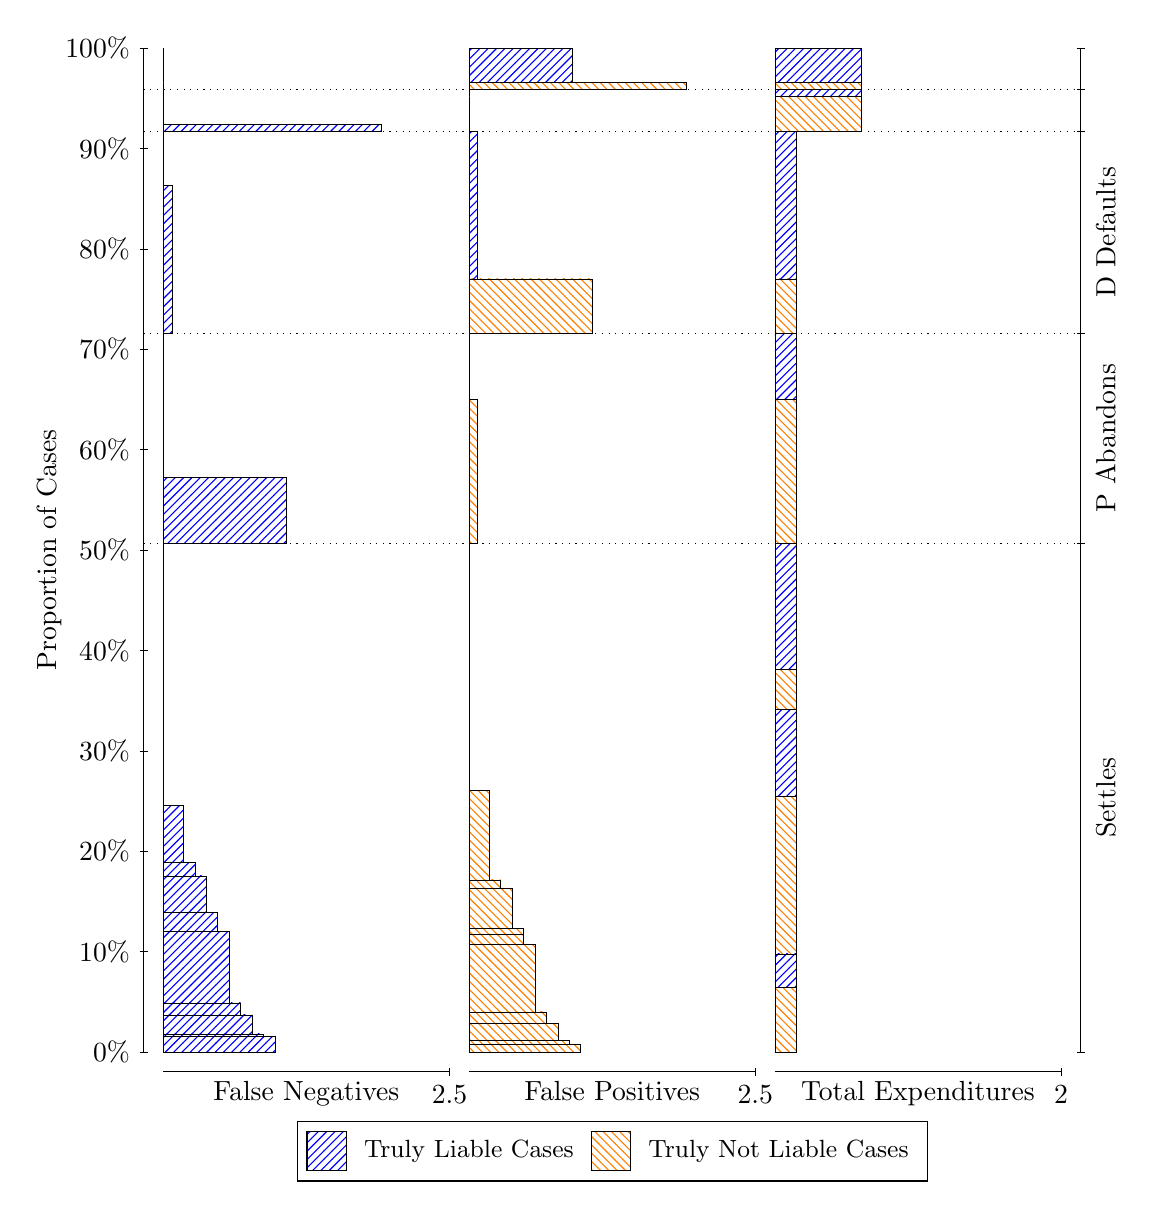
\begin{tikzpicture}
\draw[black, very thin] (1.5,1.75) -- (1.5,14.5);
\node[rotate=90, text=black, anchor=center] at (0.3, 8.125) {Proportion of Cases};
\draw[black, very thin] (1.45,1.75) -- (1.55,1.75);
\node[text=black, anchor=east] at (1.45, 1.75) {0\%};
\draw[black, very thin] (1.45,3.025) -- (1.55,3.025);
\node[text=black, anchor=east] at (1.45, 3.025) {10\%};
\draw[black, very thin] (1.45,4.3) -- (1.55,4.3);
\node[text=black, anchor=east] at (1.45, 4.3) {20\%};
\draw[black, very thin] (1.45,5.575) -- (1.55,5.575);
\node[text=black, anchor=east] at (1.45, 5.575) {30\%};
\draw[black, very thin] (1.45,6.85) -- (1.55,6.85);
\node[text=black, anchor=east] at (1.45, 6.85) {40\%};
\draw[black, very thin] (1.45,8.125) -- (1.55,8.125);
\node[text=black, anchor=east] at (1.45, 8.125) {50\%};
\draw[black, very thin] (1.45,9.4) -- (1.55,9.4);
\node[text=black, anchor=east] at (1.45, 9.4) {60\%};
\draw[black, very thin] (1.45,10.675) -- (1.55,10.675);
\node[text=black, anchor=east] at (1.45, 10.675) {70\%};
\draw[black, very thin] (1.45,11.95) -- (1.55,11.95);
\node[text=black, anchor=east] at (1.45, 11.95) {80\%};
\draw[black, very thin] (1.45,13.225) -- (1.55,13.225);
\node[text=black, anchor=east] at (1.45, 13.225) {90\%};
\draw[black, very thin] (1.45,14.5) -- (1.55,14.5);
\node[text=black, anchor=east] at (1.45, 14.5) {100\%};

\draw[black, very thin] (13.4,1.75) -- (13.4,14.5);
\draw[black, very thin] (13.35,1.75) -- (13.45,1.75);
\node[anchor=west] at (13.35, 1.75) {};
\draw[black, very thin] (13.35,8.2067) -- (13.45,8.2067);
\node[anchor=west] at (13.35, 8.2067) {};
\draw[black, very thin] (13.35,10.877) -- (13.45,10.877);
\node[anchor=west] at (13.35, 10.877) {};
\draw[black, very thin] (13.35,13.443) -- (13.45,13.443);
\node[anchor=west] at (13.35, 13.443) {};
\draw[black, very thin] (13.35,13.973) -- (13.45,13.973);
\node[anchor=west] at (13.35, 13.973) {};
\draw[black, very thin] (13.35,14.5) -- (13.45,14.5);
\node[anchor=west] at (13.35, 14.5) {};

\draw[black, very thin, pattern color=blue, pattern=north east lines] (1.75,1.75) rectangle (3.167,1.9433);
\draw[black, very thin, pattern color=blue, pattern=north east lines] (1.75,1.9433) rectangle (3.0217,1.9805);
\draw[black, very thin, pattern color=blue, pattern=north east lines] (1.75,1.9805) rectangle (2.8763,2.2204);
\draw[black, very thin, pattern color=blue, pattern=north east lines] (1.75,2.2204) rectangle (2.731,2.3739);
\draw[black, very thin, pattern color=blue, pattern=north east lines] (1.75,2.3739) rectangle (2.5857,3.2831);
\draw[black, very thin, pattern color=blue, pattern=north east lines] (1.75,3.2831) rectangle (2.4403,3.5189);
\draw[black, very thin, pattern color=blue, pattern=north east lines] (1.75,3.5189) rectangle (2.295,3.9875);
\draw[black, very thin, pattern color=blue, pattern=north east lines] (1.75,3.9875) rectangle (2.1497,4.1532);
\draw[black, very thin, pattern color=blue, pattern=north east lines] (1.75,4.1532) rectangle (2.0043,4.8826);
\draw[black, very thin, pattern color=orange, pattern=north west lines] (1.75,4.8826) rectangle (1.75,8.2067);
\draw[black, very thin, pattern color=blue, pattern=north east lines] (1.75,8.2067) rectangle (3.3123,9.0486);
\draw[black, very thin, pattern color=orange, pattern=north west lines] (1.75,9.0486) rectangle (1.75,10.877);
\draw[black, very thin, pattern color=blue, pattern=north east lines] (1.75,10.877) rectangle (1.859,12.751);
\draw[black, very thin, pattern color=orange, pattern=north west lines] (1.75,12.751) rectangle (1.75,13.443);
\draw[black, very thin, pattern color=blue, pattern=north east lines] (1.75,13.443) rectangle (4.5113,13.533);
\draw[black, very thin, pattern color=orange, pattern=north west lines] (1.75,13.533) rectangle (1.75,13.973);
\draw[black, very thin, pattern color=orange, pattern=north west lines] (1.75,13.973) rectangle (1.75,14.064);
\draw[black, very thin, pattern color=blue, pattern=north east lines] (1.75,14.064) rectangle (1.75,14.5);
\draw[black, very thin, pattern color=orange, pattern=north west lines] (5.6333,1.75) rectangle (7.0503,1.8431);
\draw[black, very thin, pattern color=orange, pattern=north west lines] (5.6333,1.8431) rectangle (6.905,1.8997);
\draw[black, very thin, pattern color=orange, pattern=north west lines] (5.6333,1.8997) rectangle (6.7597,2.1129);
\draw[black, very thin, pattern color=orange, pattern=north west lines] (5.6333,2.1129) rectangle (6.6143,2.2579);
\draw[black, very thin, pattern color=orange, pattern=north west lines] (5.6333,2.2579) rectangle (6.469,3.1193);
\draw[black, very thin, pattern color=orange, pattern=north west lines] (5.6333,3.1193) rectangle (6.3237,3.2448);
\draw[black, very thin, pattern color=orange, pattern=north west lines] (5.6333,3.2448) rectangle (6.3237,3.3231);
\draw[black, very thin, pattern color=orange, pattern=north west lines] (5.6333,3.3231) rectangle (6.1783,3.826);
\draw[black, very thin, pattern color=orange, pattern=north west lines] (5.6333,3.826) rectangle (6.033,3.9358);
\draw[black, very thin, pattern color=orange, pattern=north west lines] (5.6333,3.9358) rectangle (5.8877,5.0741);
\draw[black, very thin, pattern color=blue, pattern=north east lines] (5.6333,5.0741) rectangle (5.6333,8.2067);
\draw[black, very thin, pattern color=orange, pattern=north west lines] (5.6333,8.2067) rectangle (5.7423,10.035);
\draw[black, very thin, pattern color=blue, pattern=north east lines] (5.6333,10.035) rectangle (5.6333,10.877);
\draw[black, very thin, pattern color=orange, pattern=north west lines] (5.6333,10.877) rectangle (7.1957,11.569);
\draw[black, very thin, pattern color=blue, pattern=north east lines] (5.6333,11.569) rectangle (5.7423,13.443);
\draw[black, very thin, pattern color=orange, pattern=north west lines] (5.6333,13.443) rectangle (5.6333,13.883);
\draw[black, very thin, pattern color=blue, pattern=north east lines] (5.6333,13.883) rectangle (5.6333,13.973);
\draw[black, very thin, pattern color=orange, pattern=north west lines] (5.6333,13.973) rectangle (8.3947,14.064);
\draw[black, very thin, pattern color=blue, pattern=north east lines] (5.6333,14.064) rectangle (6.9413,14.5);
\draw[black, very thin, pattern color=orange, pattern=north west lines] (9.5167,1.75) rectangle (9.7892,2.5665);
\draw[black, very thin, pattern color=blue, pattern=north east lines] (9.5167,2.5665) rectangle (9.7892,2.9971);
\draw[black, very thin, pattern color=orange, pattern=north west lines] (9.5167,2.9971) rectangle (9.7892,4.9968);
\draw[black, very thin, pattern color=blue, pattern=north east lines] (9.5167,4.9968) rectangle (9.7892,6.0993);
\draw[black, very thin, pattern color=orange, pattern=north west lines] (9.5167,6.0993) rectangle (9.7892,6.6072);
\draw[black, very thin, pattern color=blue, pattern=north east lines] (9.5167,6.6072) rectangle (9.7892,8.2067);
\draw[black, very thin, pattern color=orange, pattern=north west lines] (9.5167,8.2067) rectangle (9.7892,10.035);
\draw[black, very thin, pattern color=blue, pattern=north east lines] (9.5167,10.035) rectangle (9.7892,10.877);
\draw[black, very thin, pattern color=orange, pattern=north west lines] (9.5167,10.877) rectangle (9.7892,11.569);
\draw[black, very thin, pattern color=blue, pattern=north east lines] (9.5167,11.569) rectangle (9.7892,13.443);
\draw[black, very thin, pattern color=orange, pattern=north west lines] (9.5167,13.443) rectangle (10.607,13.883);
\draw[black, very thin, pattern color=blue, pattern=north east lines] (9.5167,13.883) rectangle (10.607,13.973);
\draw[black, very thin, pattern color=orange, pattern=north west lines] (9.5167,13.973) rectangle (10.607,14.064);
\draw[black, very thin, pattern color=blue, pattern=north east lines] (9.5167,14.064) rectangle (10.607,14.5);
\draw[black, dotted] (1.5,8.2067) -- (13.4,8.2067);
\draw[black, dotted] (1.5,10.877) -- (13.4,10.877);
\draw[black, dotted] (1.5,13.443) -- (13.4,13.443);
\draw[black, dotted] (1.5,13.973) -- (13.4,13.973);
\draw[black, very thin] (1.75,1.5) -- (5.3833,1.5);
\node[text=black, anchor=north] at (3.5667, 1.5) {False Negatives};
\draw[black, very thin] (5.3833,1.45) -- (5.3833,1.55);
\node[text=black, anchor=north] at (5.3833, 1.45) {2.5};

\draw[black, very thin] (5.6333,1.5) -- (9.2667,1.5);
\node[text=black, anchor=north] at (7.45, 1.5) {False Positives};
\draw[black, very thin] (9.2667,1.45) -- (9.2667,1.55);
\node[text=black, anchor=north] at (9.2667, 1.45) {2.5};

\draw[black, very thin] (9.5167,1.5) -- (13.15,1.5);
\node[text=black, anchor=north] at (11.333, 1.5) {Total Expenditures};
\draw[black, very thin] (13.15,1.45) -- (13.15,1.55);
\node[text=black, anchor=north] at (13.15, 1.45) {2};

\node[text=black, centered, rotate=90] at (13.72, 4.9784) {Settles};
\node[text=black, centered, rotate=90] at (13.72, 9.5418) {P Abandons};
\node[text=black, centered, rotate=90] at (13.72, 12.16) {D Defaults};



\draw (7.449999999999999,1.5) node[draw=none] (baseCoordinate) {};
\begin{scope}[align=center]
        \matrix[scale=0.5, draw=black, below=0.5cm of baseCoordinate, nodes={draw}, column sep=0.1cm]{
            \node[rectangle, draw, minimum width=0.5cm, minimum height=0.5cm, pattern color=blue, pattern=north east lines] {}; &
            \node[draw=none, font=\small, text=black] (B) {Truly Liable Cases}; &
            \node[rectangle, draw, minimum width=0.5cm, minimum height=0.5cm, pattern color=orange, pattern=north west lines] {}; &
            \node[draw=none, font=\small, text=black] (B) {Truly Not Liable Cases}; \\
            };
\end{scope}

\end{tikzpicture}
\end{document}